%----------------------------------------------------------------------------------------
%	PACKAGES & THEMES
%----------------------------------------------------------------------------------------

\documentclass[8pt]{beamer}

\usepackage{etex}
\mode<presentation> {
\usetheme{Vilanova}
}

\usepackage[english]{babel}
\usepackage[utf8]{inputenc}
\usepackage{array}
\usepackage{graphicx}
\usepackage{booktabs}
\usepackage{amsmath,amssymb,amsthm}
\usepackage{xcolor}
\usepackage{tikz}
\usetikzlibrary{arrows}
\usepackage{pifont}
\usepackage{listings,color}

\definecolor{listcomment}{rgb}{0.0,0.5,0.0}
\definecolor{listkeyword}{rgb}{0.0,0.0,0.5}
\definecolor{listnumbers}{gray}{0.65}
\definecolor{listlightgray}{gray}{0.955}
\definecolor{listwhite}{gray}{1.0}

\AtBeginSection[]
{
\addtocounter{framenumber}{-1}
\begin{frame}
\frametitle{Outline}
\tableofcontents[currentsection]
\end{frame}}

%----------------------------------------------------------------------------------------
%	TITLE PAGE
%----------------------------------------------------------------------------------------
\title{Orfeo ToolBox}
\subtitle{Open source processing of remote sensing images (updated for 5.4)}
\author{OTB Team CNES}
\date{}

\pgfdeclareimage[height=96mm,width=128mm]{background}{images/fondsClairSansLogo}
\pgfdeclareimage[height=0.2cm]{cc}{images/CC-licence.png}
\setbeamertemplate{background}{\pgfuseimage{background}}
\pgfdeclareimage[height=0.6cm]{logoIncrust}{images/logoIncrust}
\pgfdeclareimage[height=0.6cm]{logo_cnes}{images/logo_cnes}
\logo{
\begin{tabular}{p{0.22\textwidth}p{0.58\textwidth}p{0.1\textwidth}p{0.1\textwidth}}
\href{http://www.cnes.fr}{\pgfuseimage{logo_cnes}}
& \vspace{-0.03\textwidth} \scriptsize{} % date and event here
& \href{http://creativecommons.org/licenses/by-sa/3.0/}{\pgfuseimage{cc}} & \href{http://www.orfeo-toolbox.org}{\pgfuseimage{logoIncrust}}\\
\end{tabular}
}

\titlegraphic{\vspace*{-5em}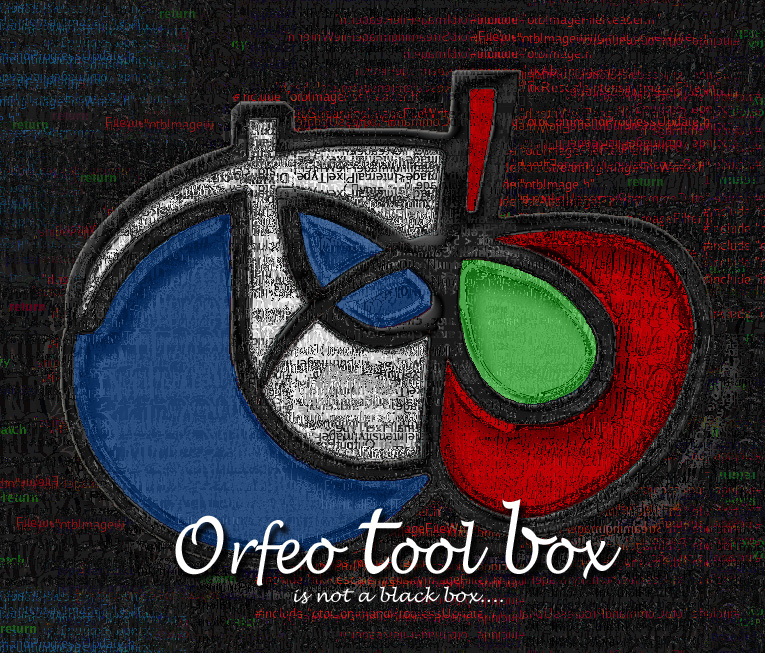
\includegraphics[width=.5\textwidth]{images/LOGOTB_blackbox.png}}

\begin{document}
\begin{frame}
\titlepage
\end{frame}

\section*{Introduction}

\begin{frame}
\frametitle{Things to know about OTB\ldots}
\begin{block}{Orfeo ToolBox is:}
\begin{itemize}
\item An \textbf{image processing library} for remote sensing
\item \textbf{Free and open source software} under CeCILL-v2 license (equivalent to GPL)
\item \textbf{Funded and developed by CNES} (French Space Agency) in the frame
  of the Orfeo Pléiades program (and beyond)
\item Written in \textbf{C++} on top of \href{www.itk.org}{ITK} (medical image
  processing)
\item Built on the shoulders of giants (GDAL, OSSIM, OpenCV\ldots)
\item \textbf{Big Data} capable, thanks to built-in streaming and multithreading
\end{itemize}
\end{block}

\begin{center}
{\huge\textcolor{red}{\href{http://www.orfeo-toolbox.org}{orfeo-toolbox.org}}}
\end{center}

\end{frame}

\begin{frame}
\frametitle{Why open source?}

\begin{block}{Maximum reach}
OTB is dedicated to every user of satellite images. Its wide
dissemination contributes to the missions sucess (Pléiades, Sentinels\ldots)
\end{block}

\begin{block}{Quality and efficiency}
OTB covers a vast panel of applications and thematic fields. Openness should:
\begin{itemize}
\item Facilitate appropriation and validation for users
\item Encourage contributions and bug reports
\item Available on multiple platforms
\item ``The Cathedral \& the
  Bazaar''\footnote{\url{http://www.catb.org/esr/writings/cathedral-bazaar/}}: the more widely available the source code is for public testing
  experimentation, the more rapidly all forms of bugs will be discovered
\end{itemize}
\end{block}

\begin{block}{Reproducible research}
OTB capitalizes a part of the CNES R\&D in IP, open source contributes to  transparent, \alert{reproducible} and trans-disciplinary \alert{research}.
\end{block}

\end{frame}

\section{Key characteristics}

\begin{frame}
\frametitle{Build on top of other open source IP software}
\begin{block}{Motivations}
\begin{itemize}
\item Interfaces seamlessly with other IP and RS open-source software\ldots
\item Reuse is powerful
\item Increase the number of functions
\item Combine tools to create hybrid data pipeline
\end{itemize} 
\end{block}

\begin{block}{OTB backbone}
\begin{itemize}
\item \href{www.itk.org}{ITK}: OTB data processing schema based on ITK \emph{pipeline}
\item \href{www.gdal.org}{GDAL} to read/write raster/vector data
\item \href{www.ossim.org}{OSSIM} sensor modelling and metadata support 
\item \href{www.opencv.org}{OpenCV} and \href{www.libsvm.org}{LibSVM} provide
  machine learning algorithms
\item \href{www.muparser.org}{MuParser} and \href{www.muparserx.org}{MuParserX}
  powerful parsing of mathematical expression(band math)
\end{itemize}
\end{block}


\end{frame}

\begin{frame}
\frametitle{Compatible (and available) on multiple plateforms}
\begin{columns}
\column{0.5\textwidth}
\begin{block}{Goal}
\begin{itemize}
\item Compile with recent versions of:
\begin{itemize}
\item GCC
\item Clang
\item MinGW
\item Visual Studio\ldots
\end{itemize}
\item Binary packages available:
\begin{itemize}
\item UbuntuGIS repository (GIS and IP software for Ubuntu)
\item Experimental Debian packages 
\item Available in  OSGeo4W (OSGeo tools on Windows)
\item Binary installers, Port and Brew formula for Mac OS X\ldots
\end{itemize}
\end{itemize}
\end{block}
\column{0.5\textwidth}
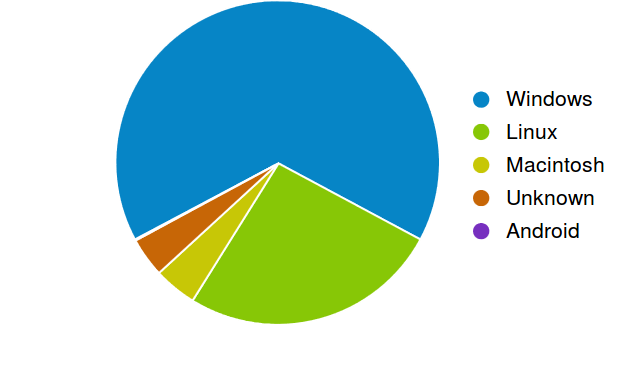
\includegraphics[width=\textwidth]{images/OTB4_download_sourceforge_os_crop.png}
\begin{center}
\tiny{Number of OTB downloads on Sourceforge per Operating System}
\end{center}
\end{columns}
\end{frame}

\begin{frame}
\frametitle{Flexibility, scalability: \textit{Pipeline}, \textit{Streaming} and \textit{multithreading}}

\begin{block}{\textit{Pipeline} data model}
\begin{center}
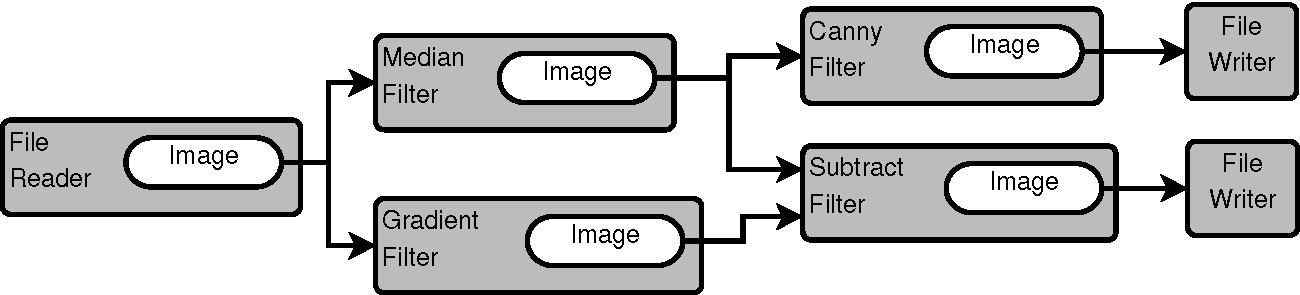
\includegraphics[width=0.7\textwidth]{images/ProcessObjectDataObject.png}
\end{center}
\end{block}
\vspace{-0.5cm}
\begin{block}{\textit{Streaming}}
\begin{center}
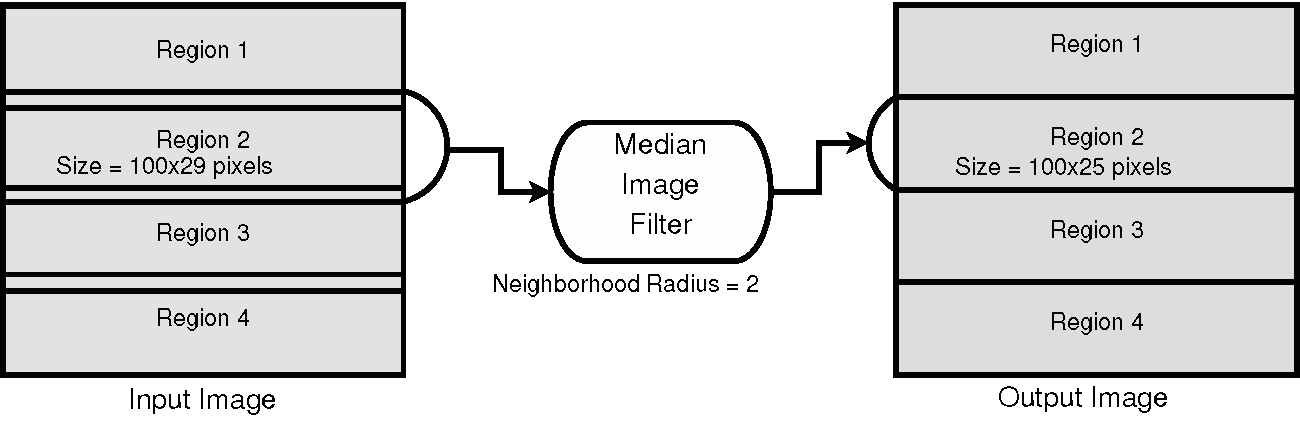
\includegraphics[width=0.7\textwidth]{images/StreamingImageDiagram.png}
\end{center}
\end{block}
\vspace{-0.5cm}
\begin{center}
\tiny{source: \url{http://www.aosabook.org/en/itk.html}}
\end{center}
\end{frame}

\begin{frame}
\frametitle{Behind the scene}
\begin{center}
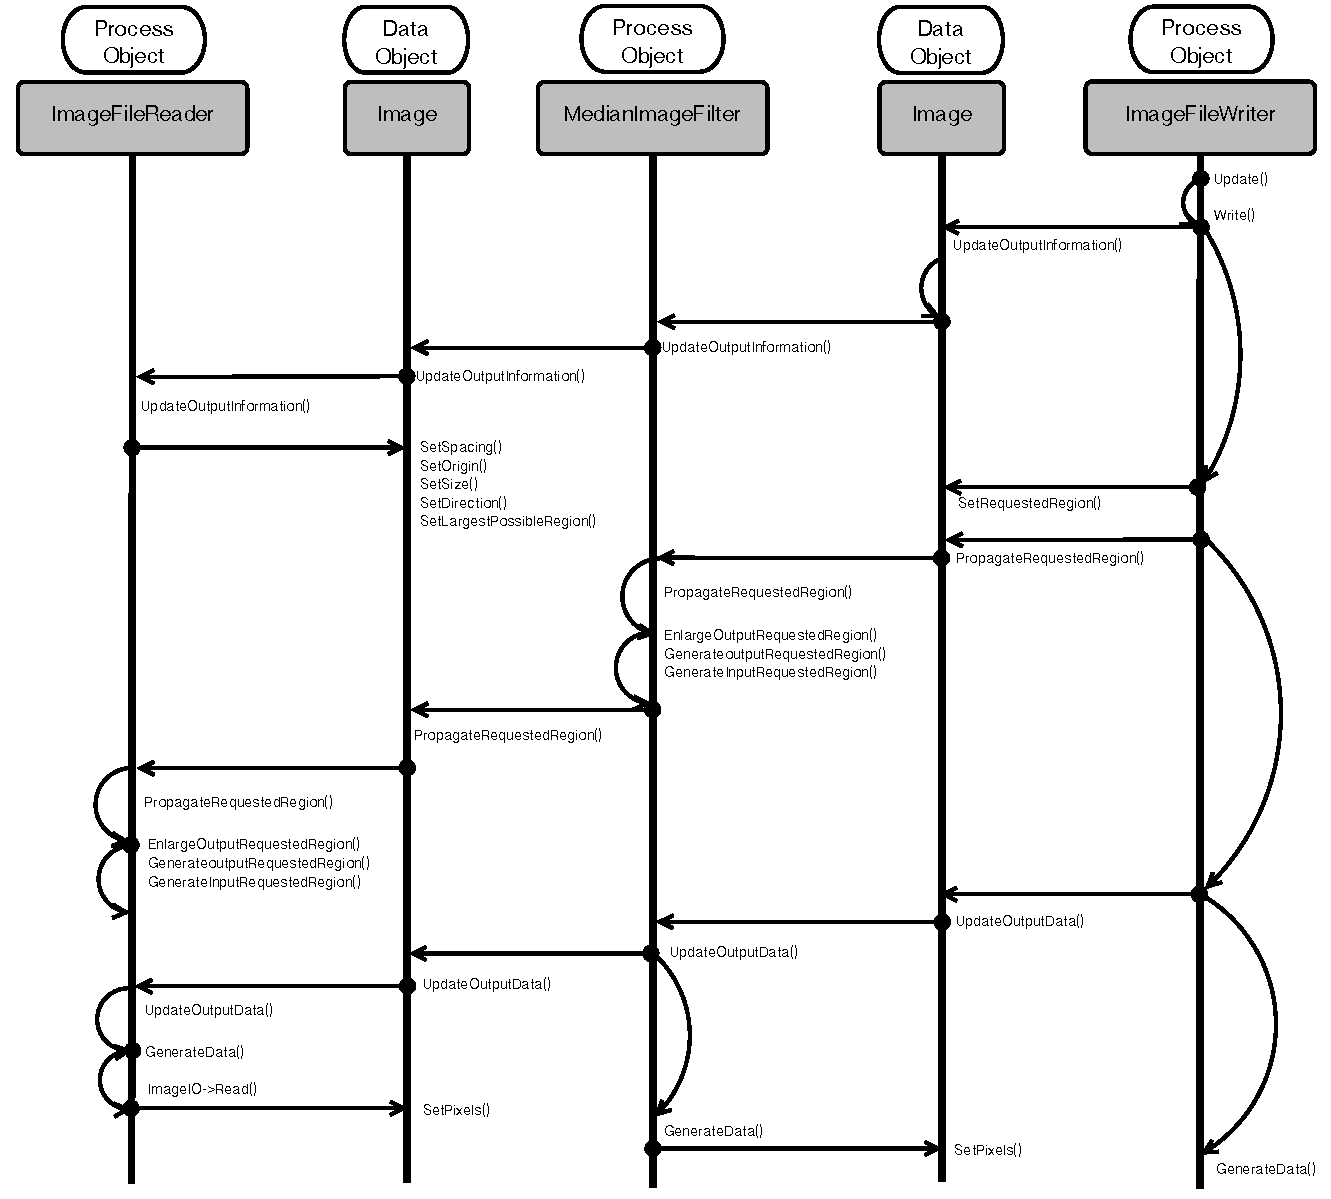
\includegraphics[width=0.7\textwidth]{images/ProcessObjectDataObjectInteractionUML.png}\\
\tiny{source: \url{http://www.aosabook.org/en/itk.html}}
\end{center}
\end{frame}

\begin{frame}
\frametitle{(Near) bleeding-edge techniques}
\begin{itemize}
\item Try to keep track of up-to-date information about the latest developments, exchanging ideas, identifying future trends, and making networking
\item Reference implementation of algorithms based on publications
\item e.g.: morphological profil,MeanShift segmentation,Haralick textures,SURF keypoints\ldots
\item Reference implementation contributes by authors with their
  publications. e.g.: Large Scale MeanShift\footnote{Michel, J.; Youssefi, D.; Grizonnet, M., "Stable Mean-Shift Algorithm and Its Application to the Segmentation of Arbitrarily Large Remote Sensing Images," Geoscience and Remote Sensing, IEEE Transactions on , vol.53, no.2, pp.952,964, Feb. 2015}, bayesian fusion\footnote{J. R. Dominique Fasbender and P. Bogaert. Bayesian data fusion for adaptable image pan-
sharpening. IEEE Transactions on Geoscience and Remote Sensing, 46(6):1847–1857, 2007.
13.2}, object detection \ldots
\end{itemize}
\end{frame}

\begin{frame}
\frametitle{How OTB is develop?}
\vspace{-0.5cm}
\begin{itemize}
\item Distributed version control: Git (migration from Mercurial in July 2015)
\item C++ and CMake(CTest, CDash)
\item Test driven development (TDD)
\item Agile (scrum)
\item Continuous integration and packaging
\end{itemize}
Every day, almost 3000 tests are compiled, launched on 16 different configurations!
\begin{center}
\href{http://dash.orfeo-toolbox.org/index.php?project=OTB}{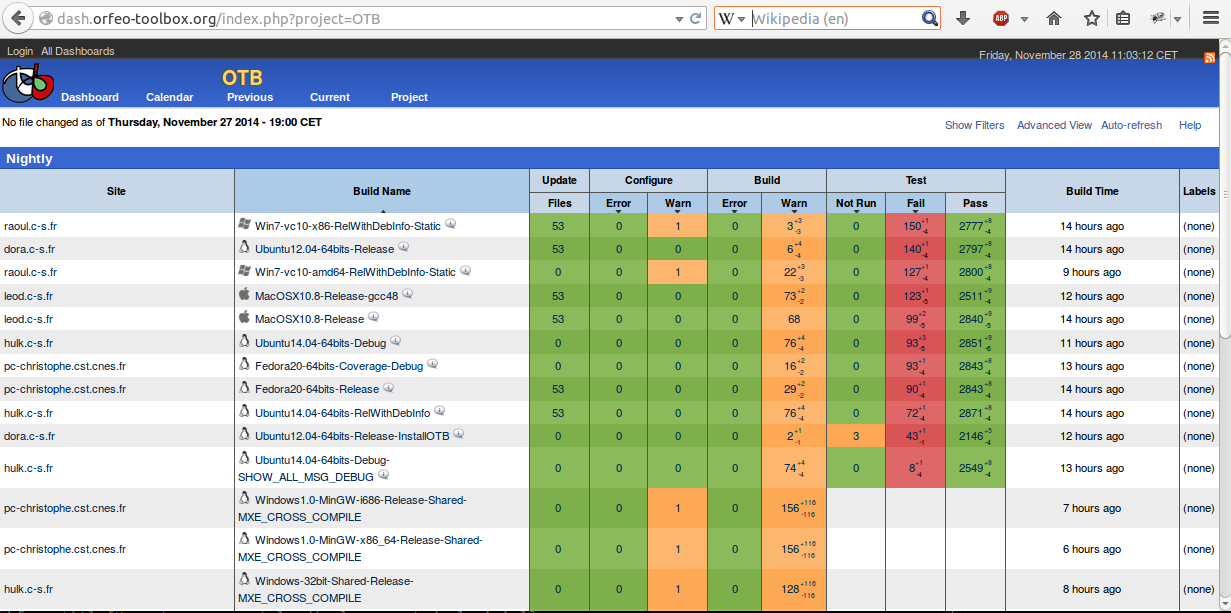
\includegraphics[width=\textwidth,trim=0 250 0 0,clip=true]{images/dashboard.png}}
\end{center}
\end{frame}

\begin{frame}
\frametitle{How to eat the OTB sandwich?}
\vspace{-0.5cm}
\begin{center}
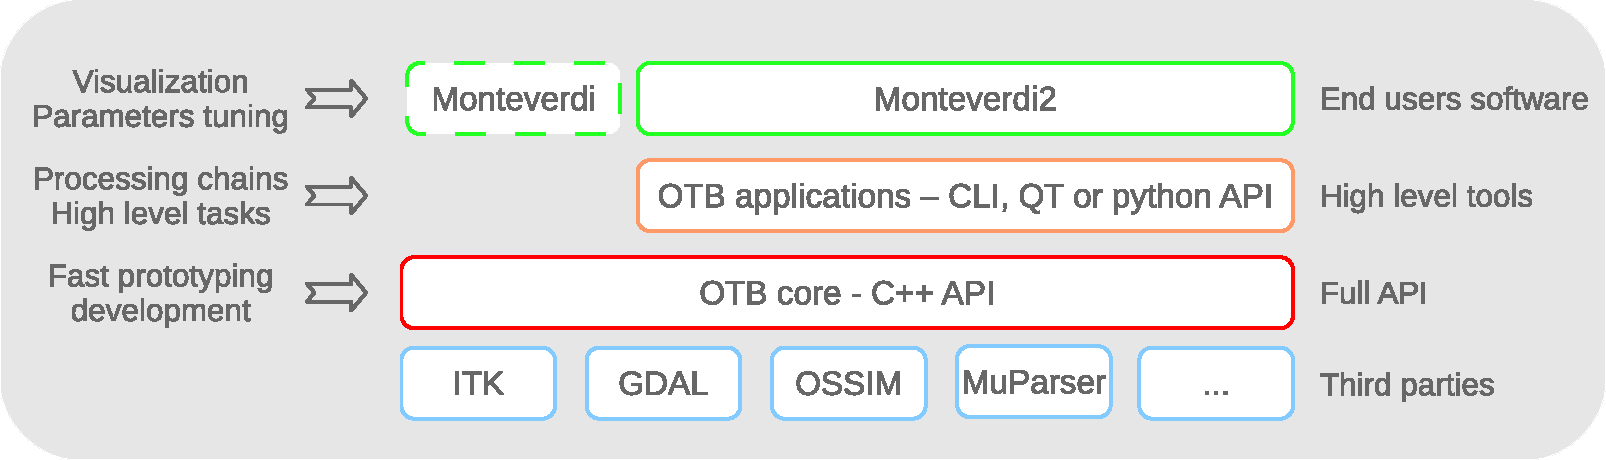
\includegraphics[width=\textwidth]{images/sandwich.pdf}
\end{center}
\vspace{-0.5cm}
\begin{block}{Write your own code}
 Flexible, access to full API, requires C++ knowledge
\end{block}
\begin{block}{Use the applications}
 High level functions (e.g. segmentation), callable from CLI, Qt, Python, can be extended
\end{block}
\begin{block}{Use Monteverdi}
Visualization, data management, \textcolor{red}{Access to all applications}
\end{block}
\end{frame}

\begin{frame}[fragile]
\frametitle{Show me the code!}
\begin{lstlisting}[language=c++,breaklines=true,breakatwhitespace=true,frame = tb,framerule = 0.25pt,fontadjust,backgroundcolor={\color{listlightgray}},basicstyle = {\ttfamily\tiny},keywordstyle = {\ttfamily\color{listkeyword}\textbf},identifierstyle = {\ttfamily},commentstyle = {\ttfamily\color{listcomment}\textit},stringstyle = {\ttfamily},showstringspaces = false,showtabs = false,numbers = none,numbersep = 2pt, numberstyle={\ttfamily\color{listnumbers}},tabsize = 2]
#include "otbImage.h"
#include "otbImageFileReader.h"
#include "otbImageFileWriter.h"
#include "itkCannyEdgeDetectionImageFilter.h"
#include "itkRescaleIntensityImageFilter.h"

int main(int argc, char * argv[])
{
  typedef double                      PixelType;
  typedef otb::Image<PixelType>       ImageType;
  
  typedef unsigned char               OutputPixelType;
  typedef otb::Image<OutputPixelType> OutputImageType;

  typedef otb::ImageFileReader<ImageType> ReaderType;
  ReaderType::Pointer reader = ReaderType::New();

  reader->SetFileName(argv[1]);

  typedef itk::CannyEdgeDetectionImageFilter
  <ImageType, ImageType> FilterType;
  FilterType::Pointer filter = FilterType::New();

  filter->SetInput(reader->GetOutput());

  typedef otb::ImageFileWriter<OutputImageType> WriterType;
  WriterType::Pointer writer = WriterType::New();

  writer->SetFileName(argv[2]);
  
  writer->SetInput(filter->GetOutput());

  writer->Update();
}
\end{lstlisting}
\end{frame}


\begin{frame}
\frametitle{The applications: write it once, use everywhere}
\begin{columns}
\column{0.5\textwidth}
\begin{itemize}
\item 87 applications are shipped with OTB
\item 1 application $=$ 1 dynamic library (plugin)
\item Applications are auto-descriptive and auto-documented
\item Applications can be extended outside of OTB
\item Several plugins players:
\begin{itemize}
  \item Command-line
  \item Qt auto-generated
  \item Python
\end{itemize}
\item Applications are meant for integration in external systems
\end{itemize}
\column{0.5\textwidth}
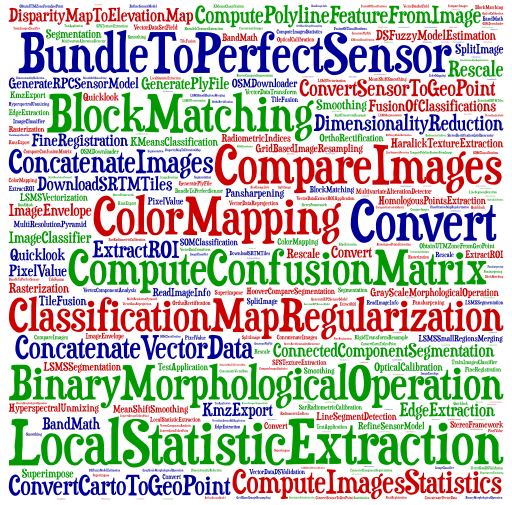
\includegraphics[width=\textwidth]{images/cloud_applications.png}
\end{columns}
\end{frame}



\begin{frame}[fragile]
\frametitle{Applications: command-line invocation}
\begin{scriptsize}
\vspace{-0.5cm}\begin{verbatim}
$ otbcli_OrthoRectification 

ERROR: Waiting for at least one parameter...
This is the OrthoRectification application, version 5.2.1
This application allows to ortho-rectify optical images from supported sensors.

Complete documentation: http://www.orfeo-toolbox.org/Applications/OrthoRectification.html

Parameters: 
        -progress                <boolean>        Report progress 
MISSING -io.in                   <string>         Input Image  (mandatory)
MISSING -io.out                  <string> [pixel] Output Image  [pixel=uint8/uint16/int16/uint32/int32/float/double] (default value is float) (mandatory)
        -map                     <string>         Output Cartographic Map Projection [utm/lambert2/lambert93/wgs/epsg] (mandatory, default value is utm)
        -map.utm.zone            <int32>          Zone number  (mandatory, default value is 31)
        -map.utm.northhem        <boolean>        Northern Hemisphere  (optional, off by default)
        -map.epsg.code           <int32>          EPSG Code  (mandatory, default value is 4326)
        -outputs.mode            <string>         Parameters estimation modes [auto/autosize/autospacing/outputroi/orthofit] (mandatory, default value is auto)
MISSING -outputs.ulx             <float>          Upper Left X  (mandatory)
MISSING -outputs.uly             <float>          Upper Left Y  (mandatory)
MISSING -outputs.sizex           <int32>          Size X  (mandatory)
MISSING -outputs.sizey           <int32>          Size Y  (mandatory)
MISSING -outputs.spacingx        <float>          Pixel Size X  (mandatory)
MISSING -outputs.spacingy        <float>          Pixel Size Y  (mandatory)
        -outputs.lrx             <float>          Lower right X  (optional, off by default)
        -outputs.lry             <float>          Lower right Y  (optional, off by default)
        -outputs.ortho           <string>         Model ortho-image  (optional, off by default)
        -outputs.isotropic       <boolean>        Force isotropic spacing by default  (optional, on by default)
        -outputs.default         <float>          Default pixel value  (optional, on by default, default value is 0)
        -elev.dem                <string>         DEM directory  (optional, off by default)
        -elev.geoid              <string>         Geoid File  (optional, off by default)
        -elev.default            <float>          Default elevation  (mandatory, default value is 0)
        -interpolator            <string>         Interpolation [bco/nn/linear] (mandatory, default value is bco)
\end{verbatim}
\end{scriptsize}
\end{frame}


\begin{frame}[fragile]
\frametitle{Applications: auto-generated Qt invocation (``Parameters tab'')}
\begin{center}
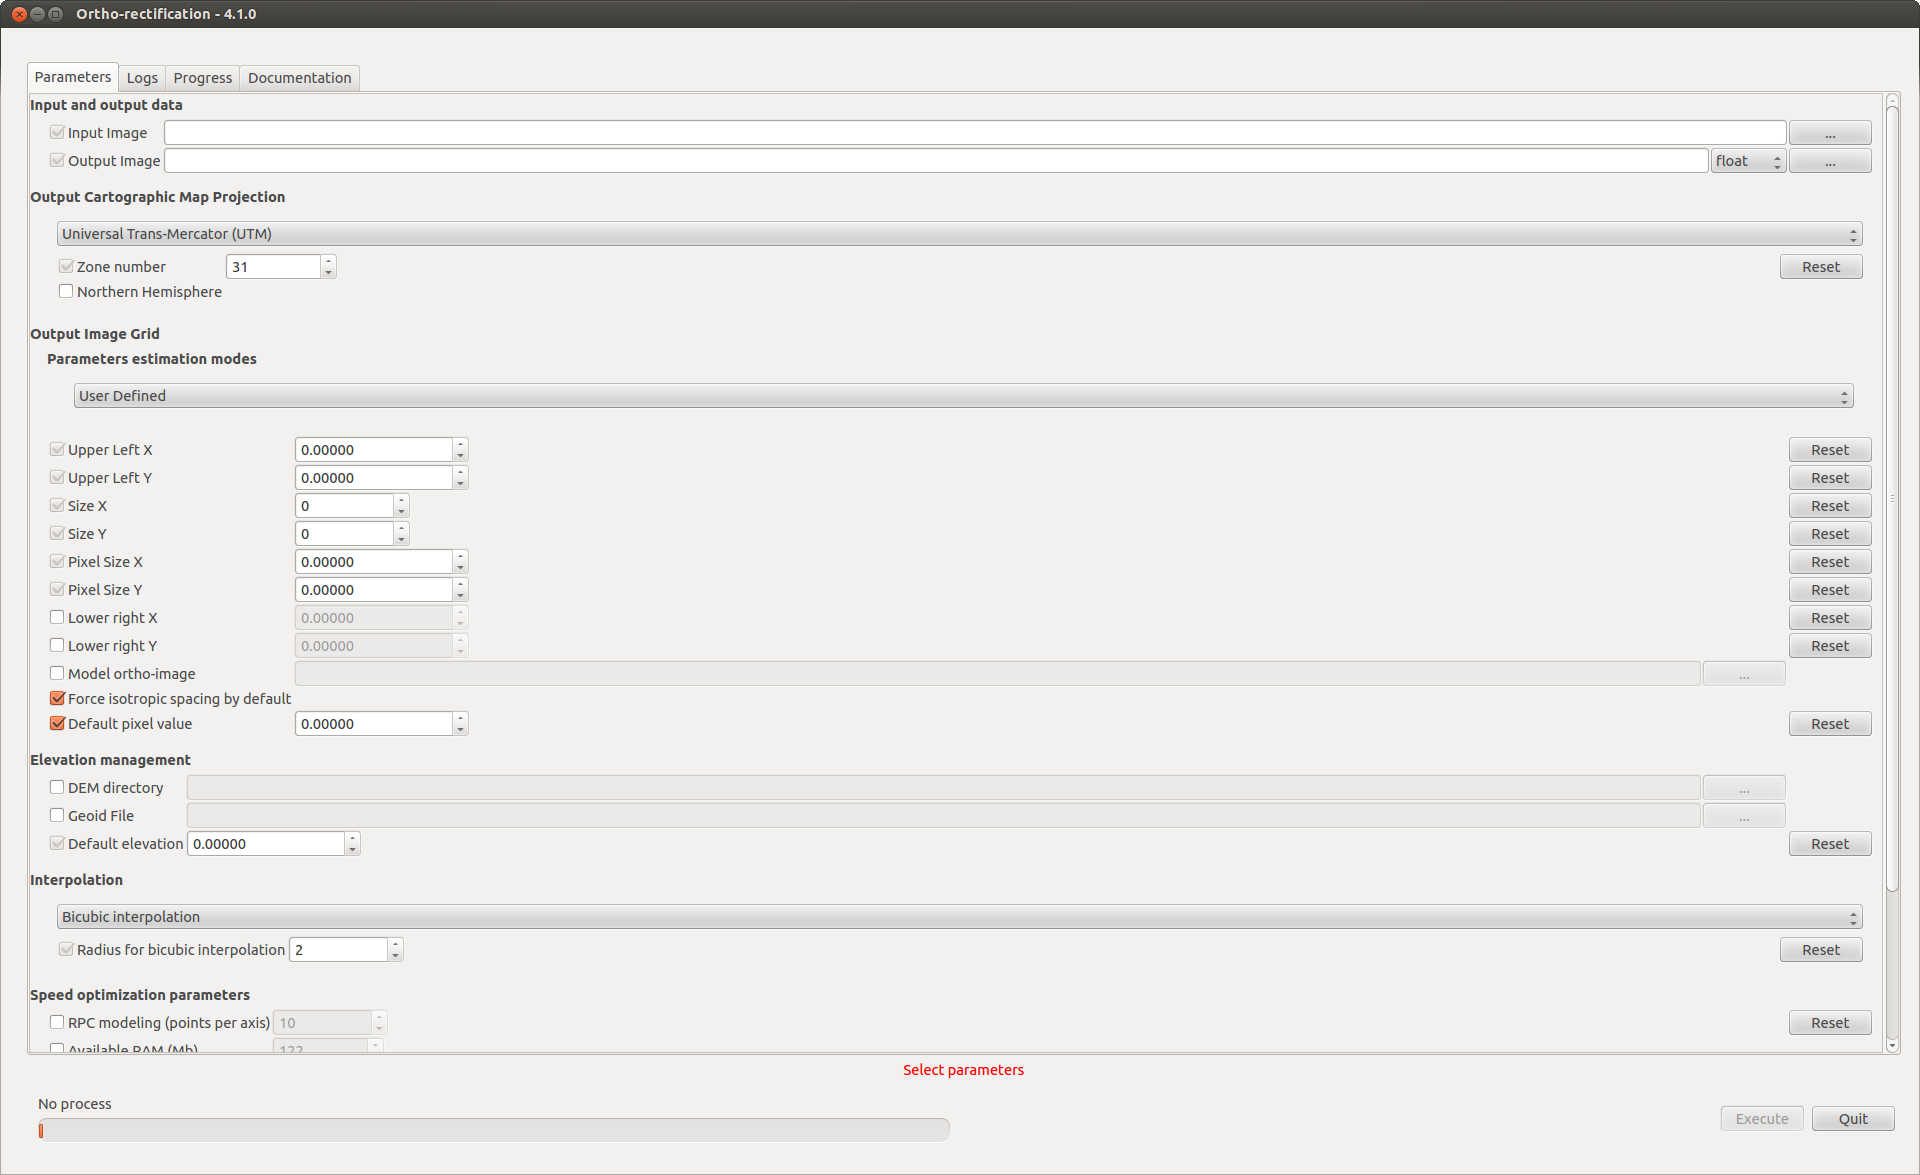
\includegraphics[width=0.9\textwidth]{images/app_parameters.png}
\end{center}
\end{frame}


\begin{frame}[fragile]
\frametitle{Applications: auto-generated Qt invocation (``Documentation tab'')}
\begin{center}
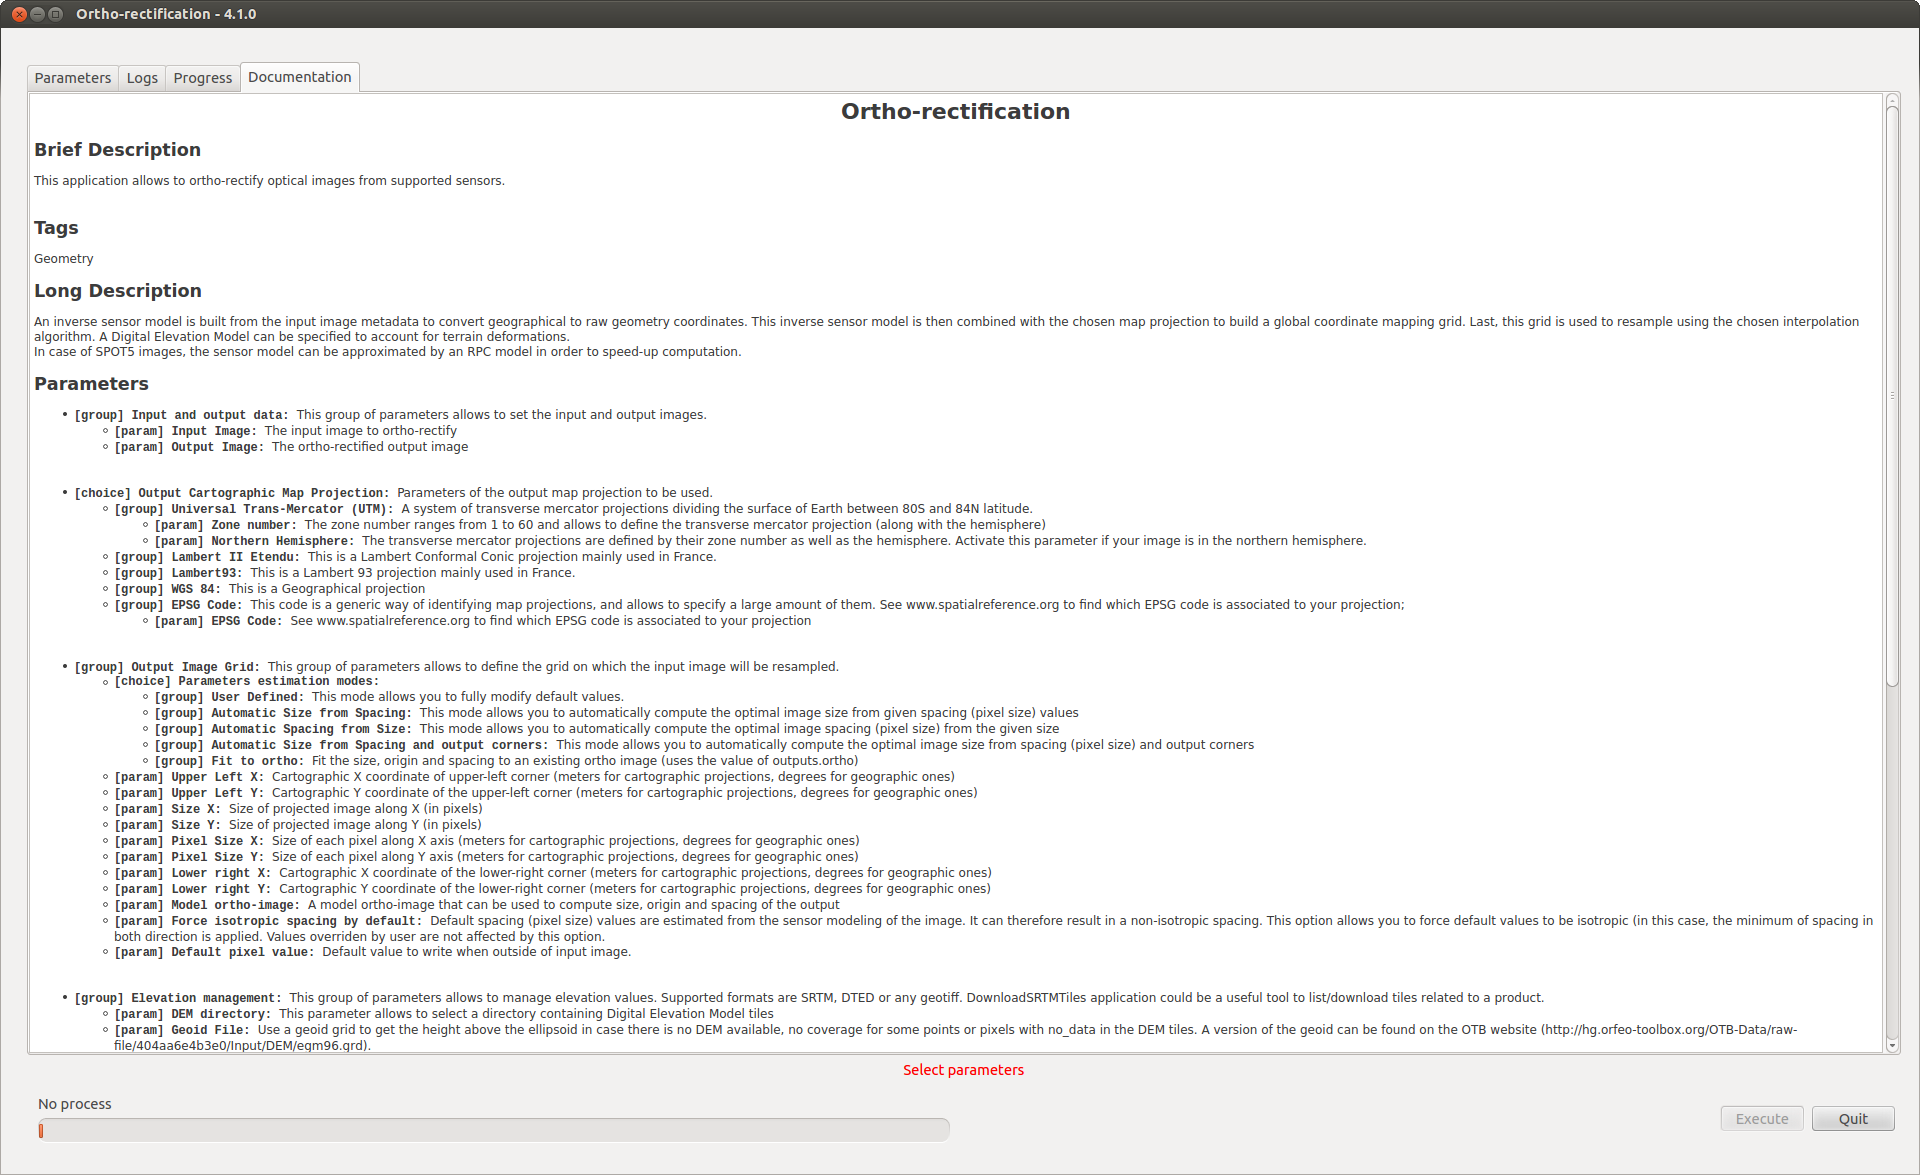
\includegraphics[width=0.9\textwidth]{images/app_doc.png}
\end{center}
\end{frame}

\begin{frame}[fragile]
\frametitle{Applications: Python wrapping}
\begin{lstlisting}[language=python,breaklines=true,breakatwhitespace=true,frame
    = tb,framerule =
    0.25pt,fontadjust,backgroundcolor={\color{listlightgray}},basicstyle =
    {\ttfamily\tiny},keywordstyle =
    {\ttfamily\color{listkeyword}\textbf},identifierstyle =
    {\ttfamily},commentstyle = {\ttfamily\color{listcomment}\textit},stringstyle
    = {\ttfamily},showstringspaces = false,showtabs = false,numbers =
    none,numbersep = 6pt, numberstyle={\ttfamily\color{listnumbers}},tabsize =
    2]
#!/usr/bin/python 
 
# Import the otb applications package 
import otbApplication 
 
# The following line creates an instance of the OrthoRectification application 
OrthoRectification = otb.Registry.CreateApplication("OrthoRectification") 
 
# The following lines set all the application parameters: 
OrthoRectification.IO.IN = "QB_TOULOUSE_MUL_Extract_500_500.tif"
OrthoRectification.IO.OUT = "QB_Toulouse_ortho.tif"
 
app.MAP = 'epsg'
app.MAP.EPSG.CODE = 32768

# The following line execute the application 
OrthoRectification.ExecuteAndWriteOutput()
\end{lstlisting}
\end{frame}


\begin{frame}
\frametitle{Monteverdi: visualization}
\begin{minipage}[t][6cm][t]{\textwidth}
\begin{center}
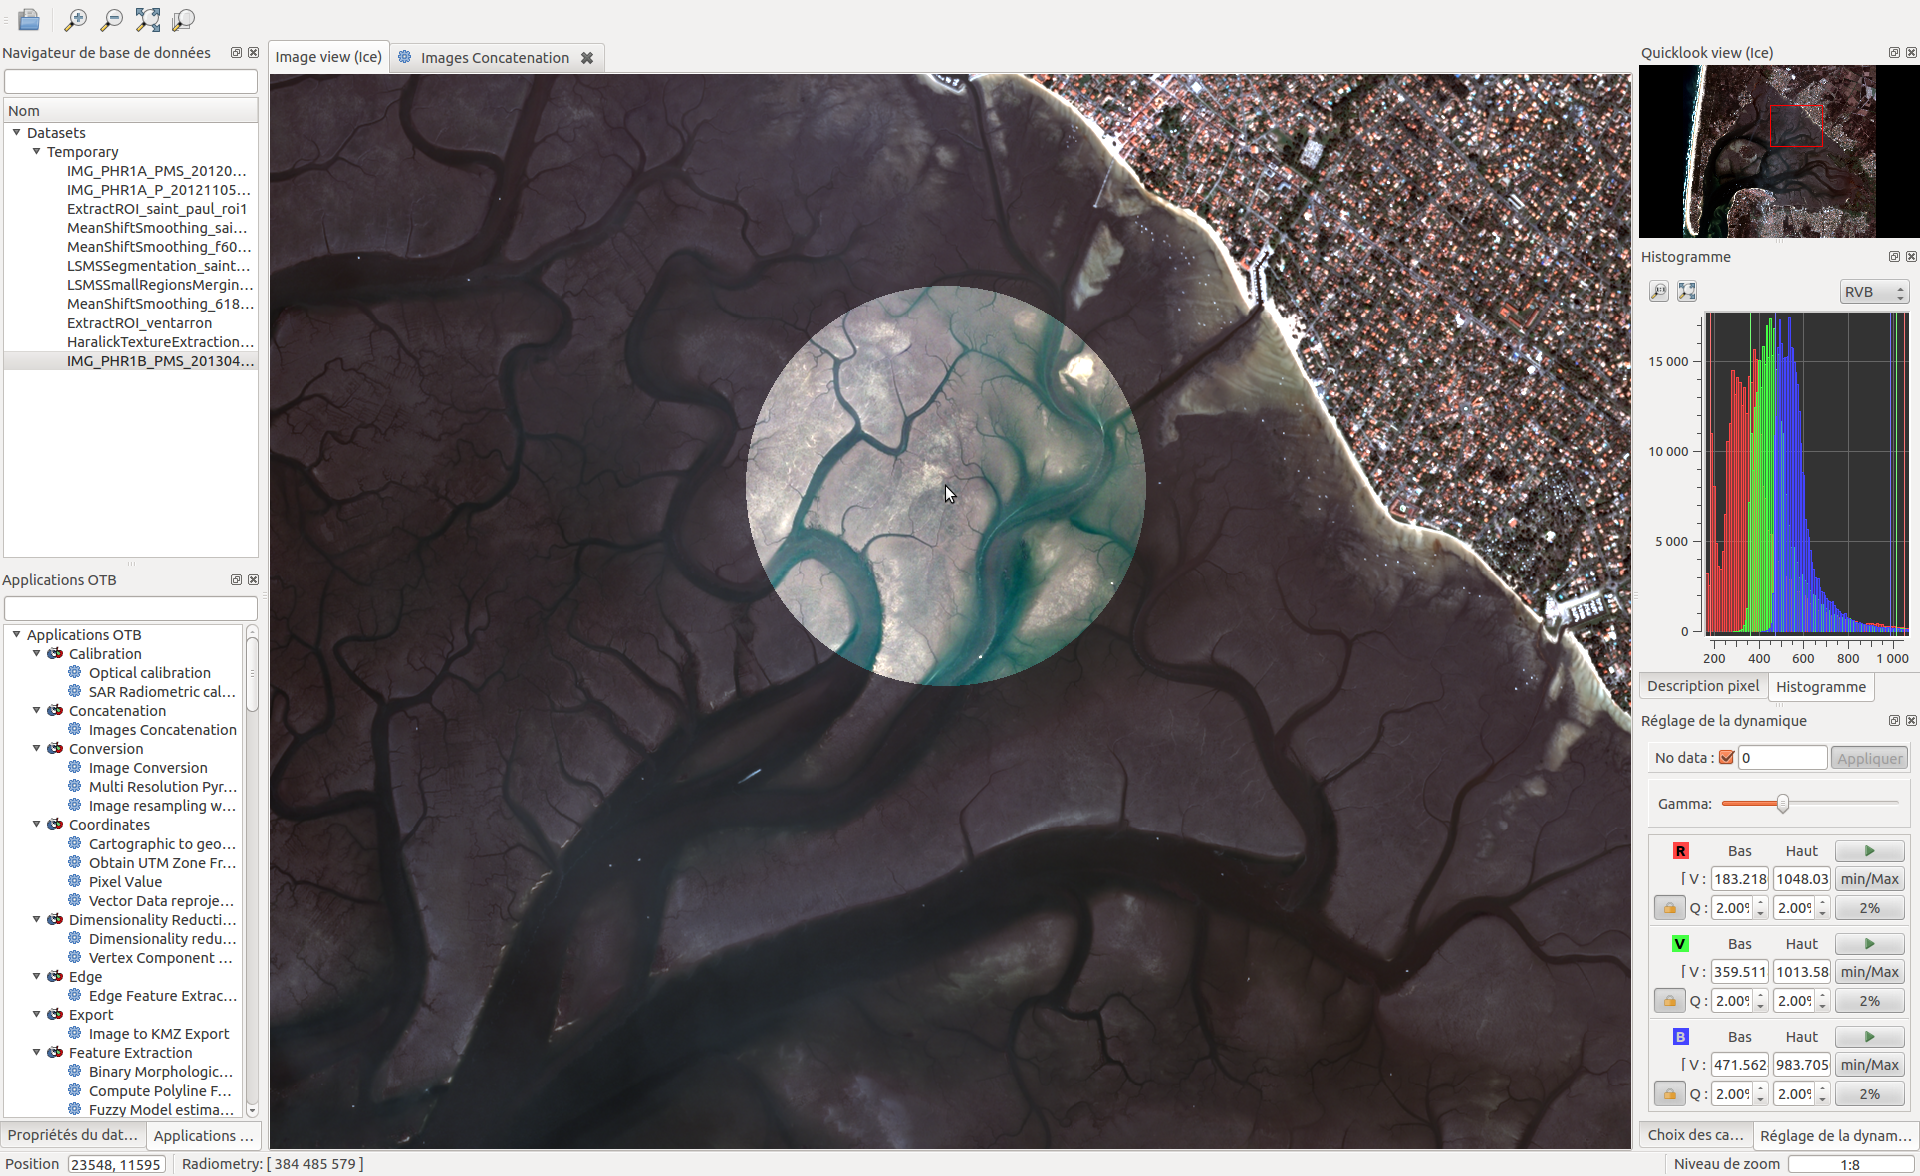
\includegraphics[width=0.9\textwidth]{images/monteverdi2-loupe.png}
\end{center}
\end{minipage}
\end{frame}

\begin{frame}
\frametitle{Monteverdi: processing}
\begin{minipage}[t][6cm][t]{\textwidth}
\begin{center}
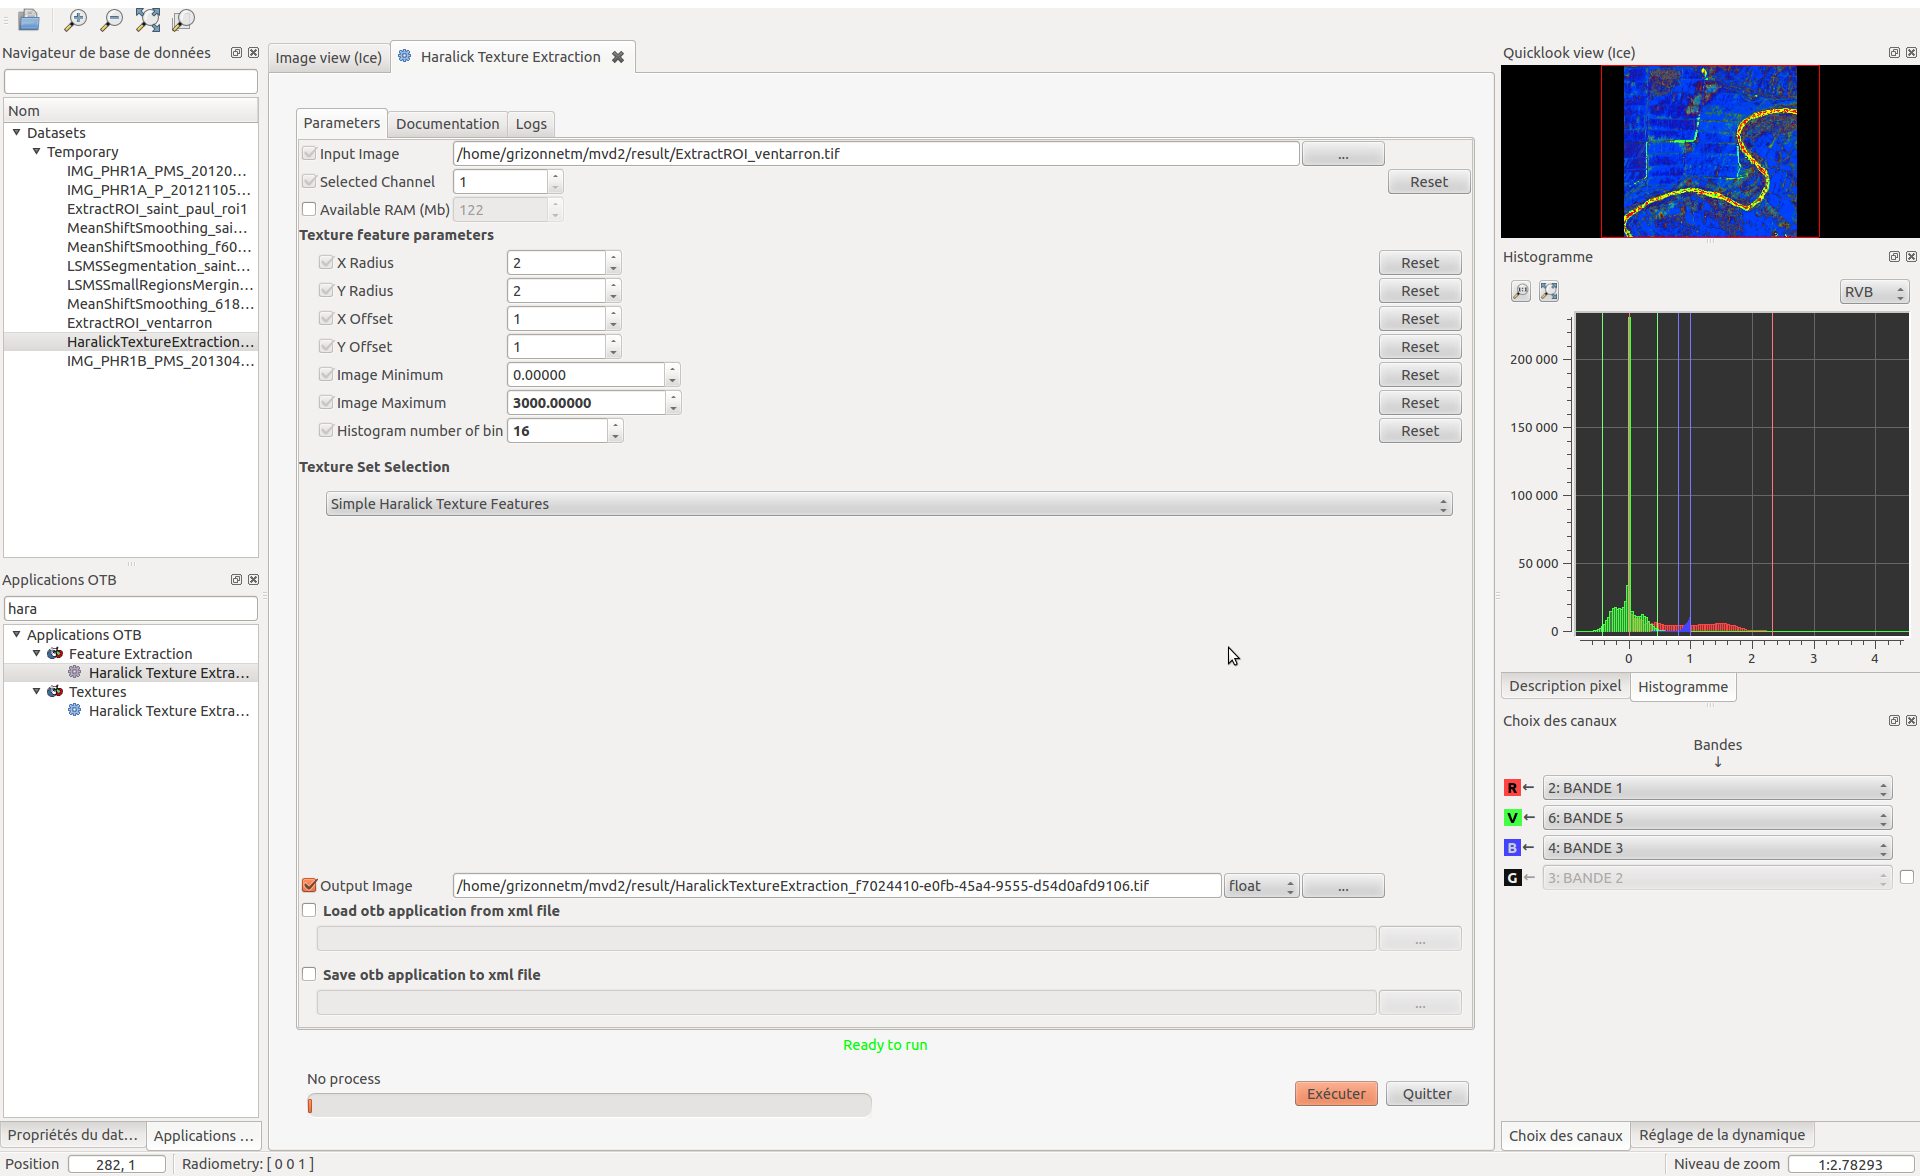
\includegraphics[width=0.9\textwidth]{images/monteverdi2-haralick.png}
\end{center}
\end{minipage}
\end{frame}

\begin{frame}
\frametitle{OTB in Quantum GIS}
\begin{minipage}[t][6cm][t]{\textwidth}
\begin{center}
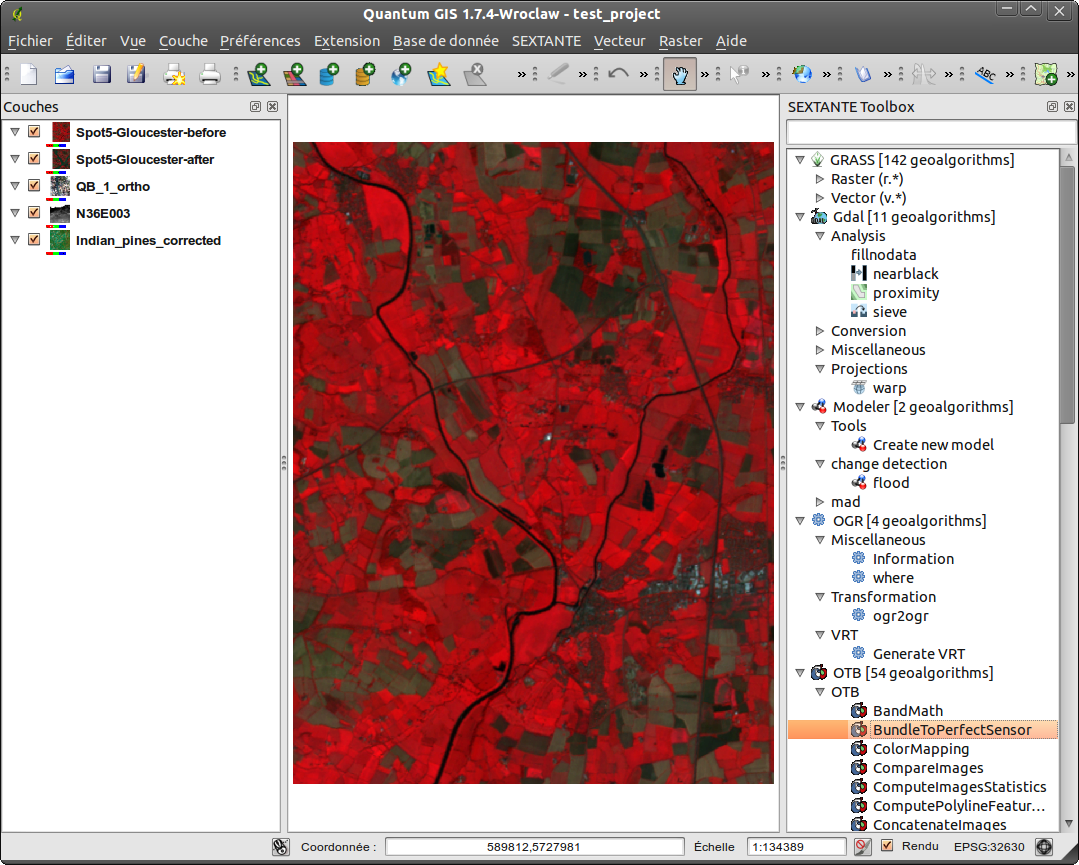
\includegraphics[width=0.7\textwidth]{images/otb_qgis.png}
\end{center}
\end{minipage}
\end{frame}

\section{Functions and algorithms}

\begin{frame}
\frametitle{Incomplete list of OTB functions}

\begin{block}{Pre-processing}
\begin{itemize}
\item Radiometric calibration, orthorectification, resampling (raster and
  vector), pan-sharpening, stereo rectification\ldots
\item Sensor supported: Sentinels, Pléiades, SPOT6, SPOT5, Digital Globe satellites
\item Geometric models (thanks to OSSIM), support for DEM (SRTM or GeoTIFF)
\end{itemize}
\end{block}

\begin{block}{Images and vector manipulation}
\begin{itemize}
\item Formats supported by GDAL (raster and vector), conversion raster/vector
\item Region of interest extraction, of spectral bands, concatenation or splitting\ldots
\item Band math, color mapping, contrast enhancement
\item Linear filtering, Mathematical morphology
\end{itemize}
\end{block}
\end{frame}

\begin{frame}
\frametitle{(Incomplete) List of OTB functions}

\begin{block}{Feature extraction}
\begin{itemize}
\item Edge detection, scale-invariant feature transform, lines, corners
\item Radiometric indices, textures (Haralick, SFS, PanTex)
\item Local statistics (Flusser moments, Histogram of Oriented Gradient)
\item Keypoints matching (SIFT, SURF\ldots)
\end{itemize}
\end{block}

\begin{block}{Change detection}
\begin{itemize}
\item Classic methods with image metrics comparison
\item Multivariate Alteration Detector
\end{itemize}
\end{block}

\begin{block}{Dimensionality reduction, hyperspectral processing}
\begin{itemize}
\item PCA, NAPCA, ICA, MAF\ldots
\item Dimension estimation, endmembers extraction, Vertex Component Analysis(VCA)
\end{itemize}
\end{block}

\end{frame}

\begin{frame}
\frametitle{Incomplete list of OTB functions}
\begin{block}{Segmentation}
\begin{itemize}
\item Segmentation algorithms: Connected Components, MeanShift,Watershed\ldots
\item Methods to apply those algorithms on large dataset
\item Vector or raster representation which allow Object Based Image Analysis
\end{itemize}
\end{block}

\begin{block}{Classification}
\begin{itemize}
\item 9 supervised methods available (including SVM and Random Forests)
\item Fusion and regularization of classifications
\item K-Means clustering or Kohonen maps
\item Object classification (from a segmentation)
\end{itemize}
\end{block}

\end{frame}

\vspace*{-6.5mm}    
\begin{frame}[plain]
\hspace*{-11mm}
    \includegraphics[keepaspectratio,height=1.1\paperheight]{images/mayotte2012.png}
\end{frame} 

\vspace*{-6.5mm}    
\begin{frame}[plain]
\hspace*{-11mm}
    \includegraphics[keepaspectratio,height=1.1\paperheight]{images/mayotte2013.png}
\end{frame} 

\vspace*{-6.5mm}    
\begin{frame}[plain]
\hspace*{-11mm}
    \includegraphics[keepaspectratio,height=1.1\paperheight]{images/mayotte_mad.png}
\end{frame} 

\vspace*{-6.5mm}    
\begin{frame}[plain]
\hspace*{-11mm}
\includegraphics[keepaspectratio,height=1.1\paperheight]{images/saint_paul_lsd.png}
\end{frame} 

\vspace*{-6.5mm}    
\begin{frame}[plain]
\hspace*{-11mm}
    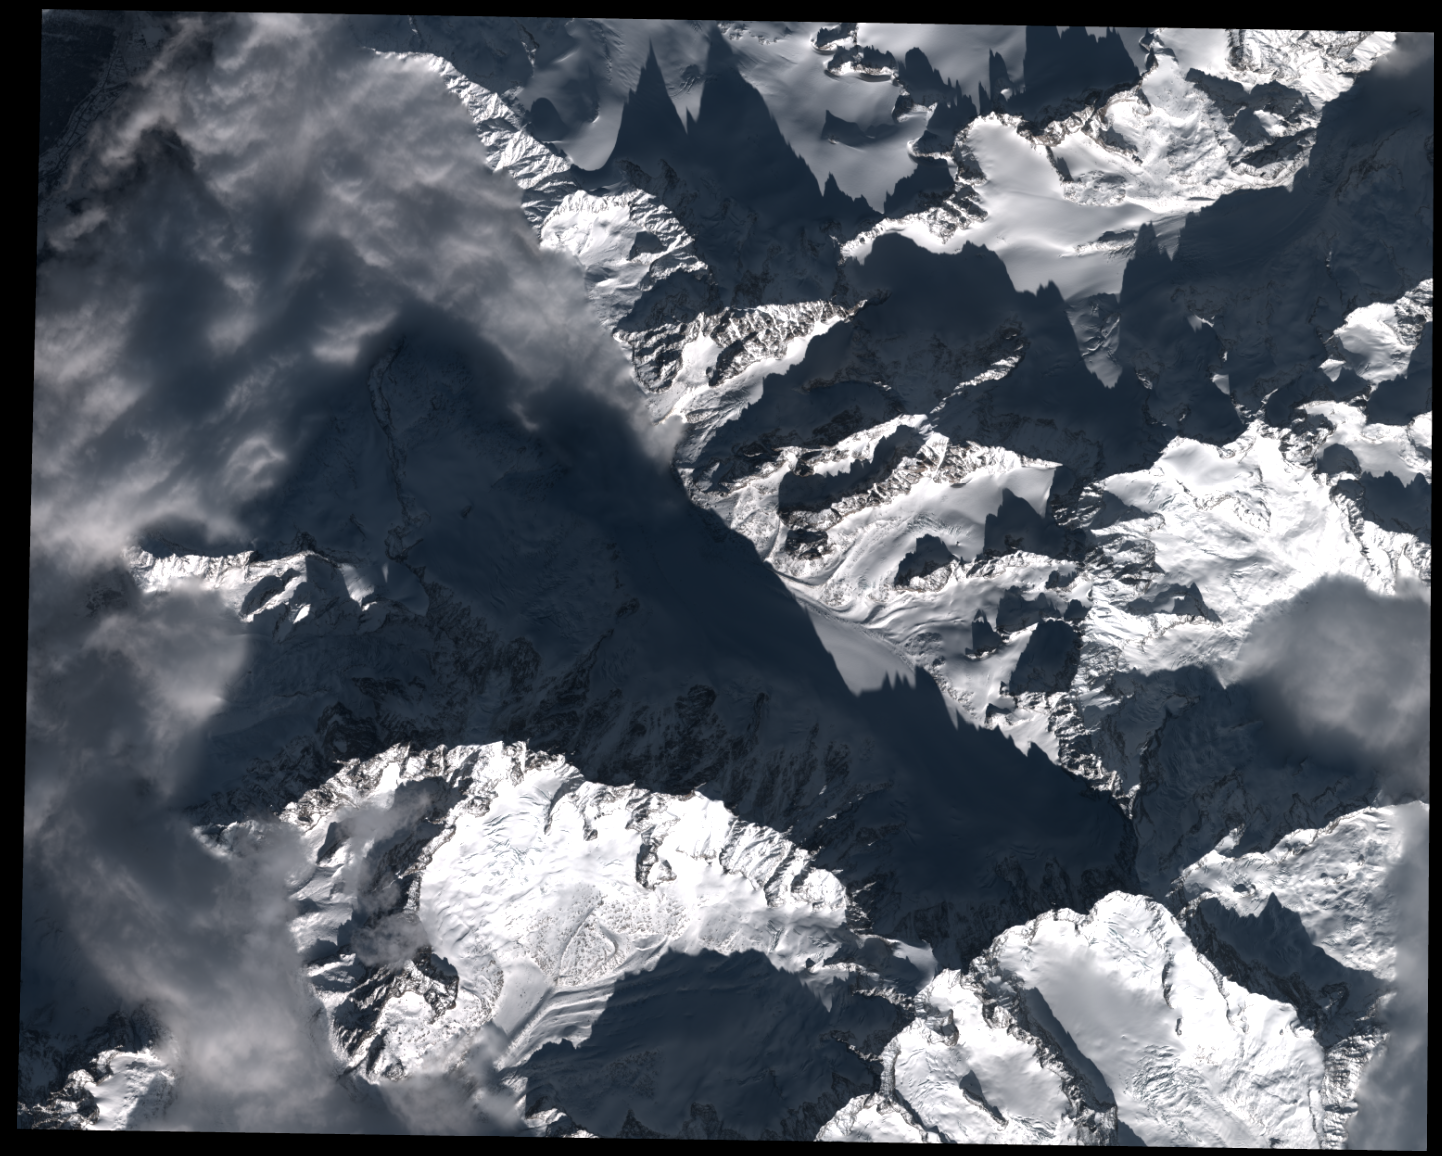
\includegraphics[keepaspectratio,width=1.005\paperwidth,height=1.1\paperheight]{images/argentiere_left.png}
\end{frame} 

\vspace*{-6.5mm}    
\begin{frame}[plain]
\hspace*{-11mm}
    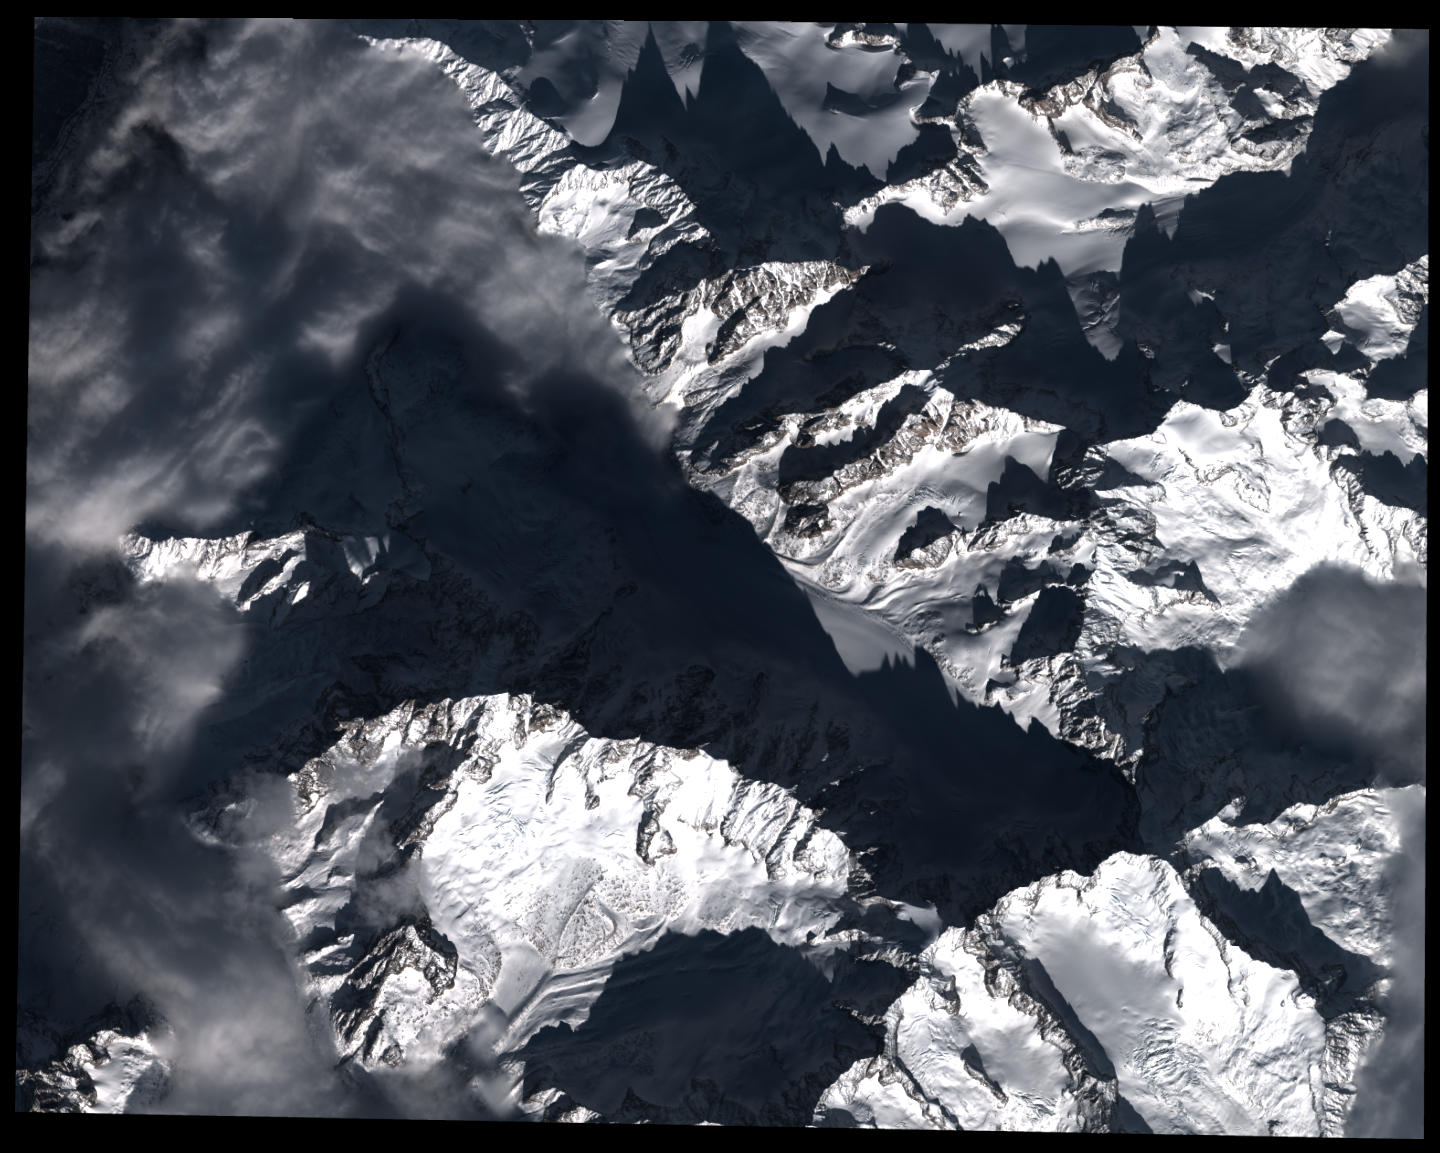
\includegraphics[keepaspectratio,width=1.005\paperwidth,height=1.1\paperheight]{images/argentiere_right.png}
\end{frame} 

\vspace*{-6.5mm}    
\begin{frame}[plain]
\hspace*{-11mm}
    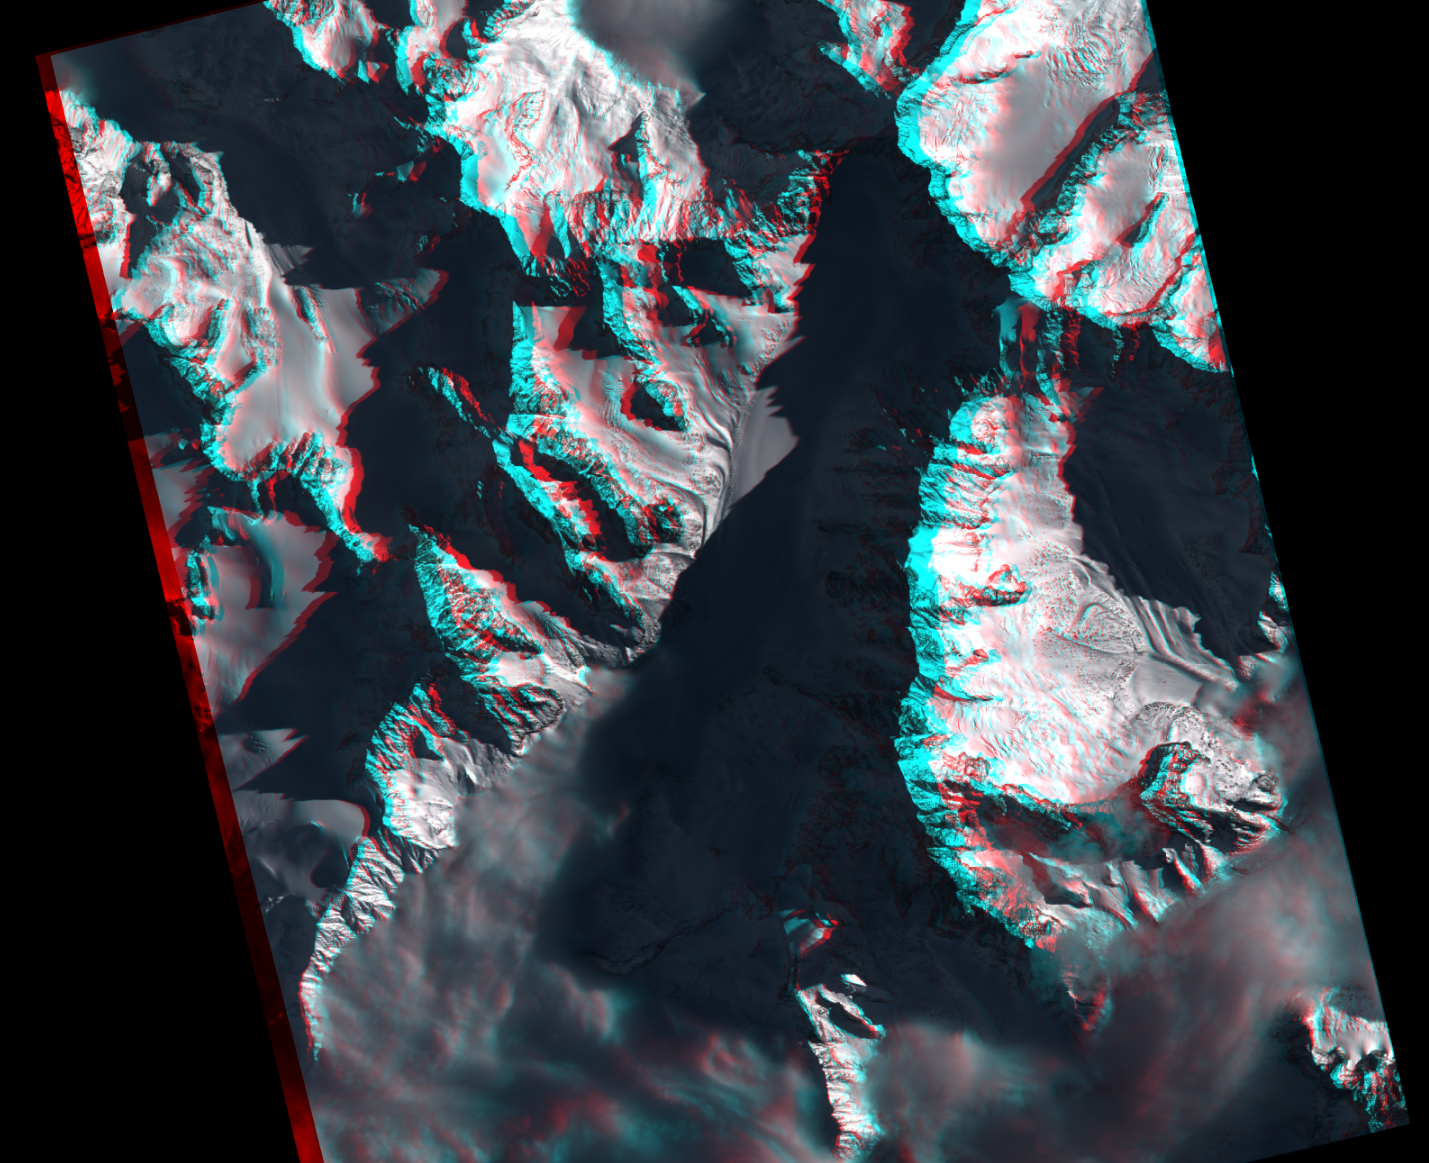
\includegraphics[keepaspectratio,width=1.005\paperwidth,height=1.1\paperheight]{images/argentiere_anaglyphe.png}
\end{frame} 

\section{What's new in OTB?}

\begin{frame}
\frametitle{Modular architecture (inspired by ITK 4.x)}
\begin{block}{What has changed?}
\begin{itemize}
\item  Organize the code into conceptual cohesive groups:
  \begin{itemize}
    \item OTB 4.4: 1672 files in 26 directories
    \item OTB 5.0: 1627 files in 124 \textbf{modules} divided in 16 groups
  \end{itemize}
\item Modules contain: tests, source code, applications are grouped
\item Each module can be (de)activate, with automatic dependencies resolutions
\item Good start! Already many remote modules contributed by the community: \url{https://www.orfeo-toolbox.org/external-projects/}
\end{itemize}
\end{block}

\begin{block}{Advantages?}
\begin{itemize}
\item Third part dependencies are integrated as modules and can be excluded
\item Lots of CMake magic (less code for configuration, better support)
\item Doxygen API documentation follows the new code organization (easier to
  find class info)
\item Facilitate external contributions with powerful mechanisms call
  \href{https://www.orfeo-toolbox.org/external-projects/}{\alert{remote module}}
\end{itemize}
\end{block}
\end{frame}

\begin{frame}
\frametitle{Contribute a module}
\begin{center}
 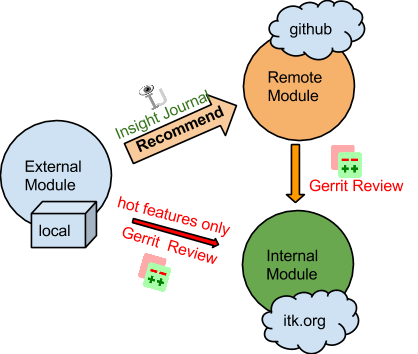
\includegraphics[width=0.4\textwidth]{images/itk-remote-module.png}
\end{center}
\end{frame}

\begin{frame}
\frametitle{Superbuild: installing OTB has never been so easy}
\begin{block}{Before in OTB 4.4}
\begin{itemize}
\item Some of the OTB third part dependencies could be build internally
\item External source code was integrated in OTB source tree (not a good idea)
\end{itemize}
\end{block}

\begin{block}{In OTB 5.0, on Superbuild!}
\begin{itemize}
\item No more third party library sources integrated in OTB
\item External project called \textbf{superbuild} which allows to
  download/configure/build/install OTB and all dependencies in one pass!
\item Allow to build OTB on an (almost) empty platform (CMake, GCC, zlib, curl),
  and everything is automatic\ldots
\item There is also an \textit{offline} mode which does not require Internet
\end{itemize}
\end{block}
\end{frame}

\begin{frame}
\frametitle{Project Steering Committee: OTB governance structure}
\begin{itemize}
\item Open governance
\item High level guidance and coordination for the ORFEO ToolBox
\item Animation of OTB community, communication, orientation of the project
\item Everyone can participate
\item All members have equal standing and voice in the PSC (1 member = 1 vote)
\item Proposals are written up and submitted on the otb-developers mailing list for discussion and voting
\item Status and decision process are
  public\footnote{\url{http://wiki.orfeo-toolbox.org/index.php/Project_Steering_Committee}}
\item Note that the PSC is not a legal entity!
\end{itemize}
\end{frame}

\begin{frame}
\frametitle{Contribute a module}
\begin{block}{ITK schema}
\begin{center}
 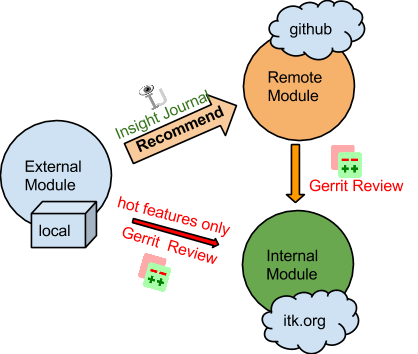
\includegraphics[width=0.4\textwidth]{images/itk-remote-module.png}
\end{center}
\end{block}
\end{frame}

\begin{frame}
\frametitle{Superbuild: installing OTB has never been so easy}
\begin{block}{Before in OTB 4.4}
\begin{itemize}
\item Some of the OTB third part dependencies could be build internally
\item External source code was integrated in OTB source tree (not a good idea)
\end{itemize}
\end{block}
\end{frame}

\begin{frame}
\frametitle{What's new in OTB 5.2?}
\begin{block}{What has changed?}
\begin{itemize}
\item New applications for SAR processing (polarimetry)
\item Basic support of Sentinel1 products
\item Radiometric calibration of Sentinel1 and Radarsat2
\item New methods for SAR Despeckle filtering (Frost, Lee, GammaMAP, Kuan)
\item Regression mode in machine learning and confidence maps for classification
\item Enhanced syntax of applications python API
\item Compatibilty with Gdal 2.0 and support of Sentinel-2
\end{itemize}
\end{block}

\begin{block}{Goodbye Monteverdi2, welcome Monteverdi 3.0}
\begin{itemize}
\item Light stack-layer model
\item Display several images together, as a stack or as a mosaic
\item Lots of nice rendering tools
\item Access to OTB applications
\end{itemize}
\end{block}
\end{frame}

\section{Conclusion}
\begin{frame}
\frametitle{How many users?}
\begin{columns}[c]
\column{0.5\textwidth}
\begin{block}{Hard to tell\ldots}
\begin{itemize}
    \item $\approx$ 600 members on the otb-users list
    \item Between 100 and 150 mails by months
    \item $\approx$ 100 members on the developers list
    \item $\approx$ 118 user accounts on the bug tracker
    \item $\approx$ 50 contributors in the documentation
    \item $\approx$ 3400 downloads for OTB 5.0 on SourceForge(released June 1, 2015).
  \end{itemize}
\end{block}
\column{0.5\textwidth}
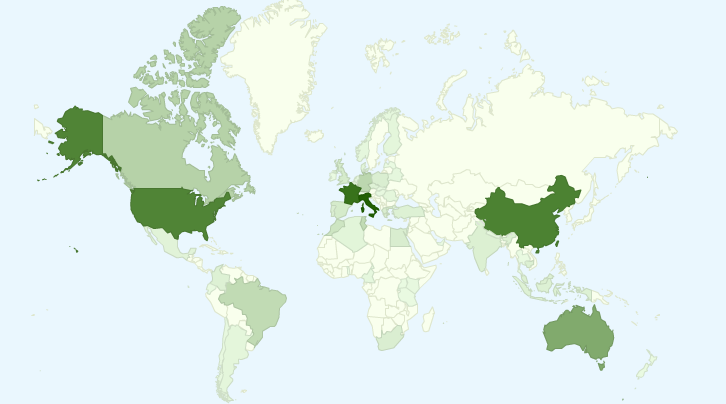
\includegraphics[width=\textwidth]{images/OTB4_download_sourceforge_country_crop.png}
\end{columns}
\end{frame}

\begin{frame}
\frametitle{Success stories}
\begin{columns}
\column{0.6\textwidth}
\begin{itemize}
\item OTB has been useful for (some) ORFEO users!
\item Several training courses (3/5-day courses) given in France, Belgium,
Madagascar, UNESCO, Hawaii,Finland\ldots
\item OTB has successfully processed 619 Pléiades
  images on RTU web site
\item OTB provides many useful RS functions in \textbf{one single tool}
\item OTB is/was the only open-source supporting PHR images (thanks to OpenJPEG)
\item OTB equals or beats state-of-the-art tools (open source and maybe \$\$) on some points: 
  \begin{itemize}
  \item band calculator
  \item tile-wise segmentation of full imagery
  \item full scene classification with a range of machine learning algorithms
  \item bridges between RS and SIG \ldots
  \end{itemize}
\item Beyond Orfeo, OTB is already used in several projects and software
\item OSGeo incubation
\end{itemize}
\column{0.4\textwidth}
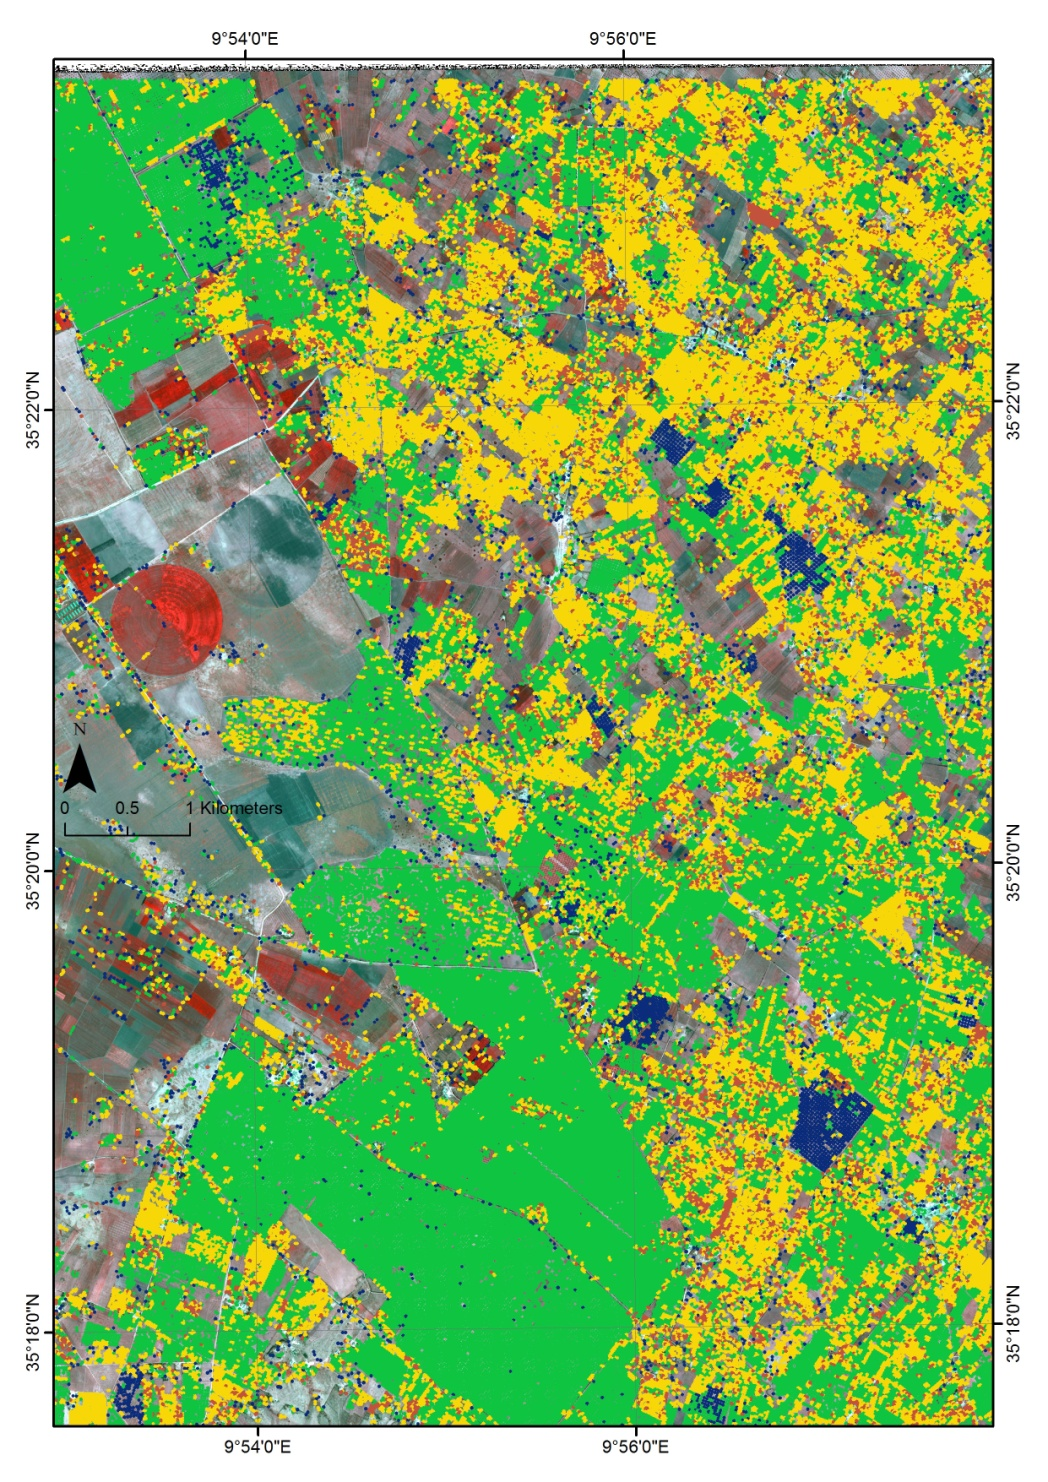
\includegraphics[width=0.9\textwidth]{images/resultats_ird.png}\\
\tiny{Thematic map from OTB segmentation, B. Mougenot~-~IRD}
\end{columns}
\end{frame}

\begin{frame}
\frametitle{Projects and software using OTB}
\begin{columns}
  \column{0.5\textwidth}
  \begin{itemize}
    \item OTB applications are available through QGIS processing framework
    \item OTB is a component of \alert{Sentinel-2} and Venus ground segment (CNES and ESA)
    \item Terr'Image: Educational software for satellite image analysis
    \item Use to prototype \alert{THEIA} products from the Scientific Expertise Centres
    \item ESA Sentinel-2 for Agriculture 
    \item Gnorasi Software (National Technical University of Athens)
    \item Vahine project (hyperspectral processing of astrophysics),IPAG
    \item Geosud project(IRSTEA)
    \item TCM research program (ETS Quebec)
  \end{itemize}
  \column{0.65\textwidth}
  \begin{center}
  \includegraphics[width=0.6\textwidth,height=0.35\textheight]{images/Carte_17Classes.png}\\
  \tiny{Prototype of THEIA Land cover product(CESBIO)}
  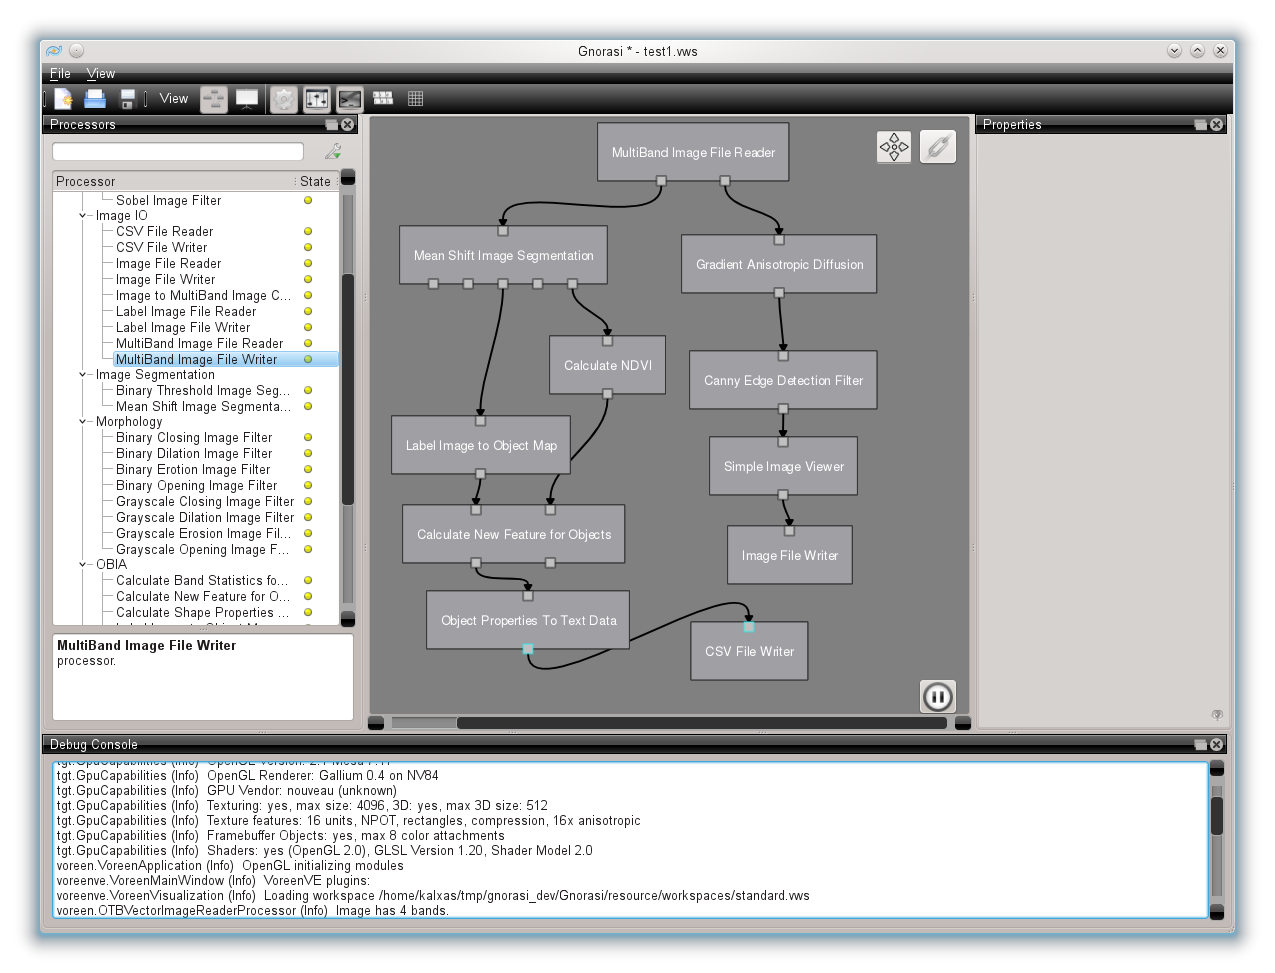
\includegraphics[width=0.6\textwidth,height=0.35\textheight]{images/gnorasi2.png}\\
  \tiny{The Gnorasi software}
  \end{center}
\end{columns}
\end{frame}

\begin{frame}
\frametitle{A complex system for complex tasks: chaos and side effects}
\begin{center}
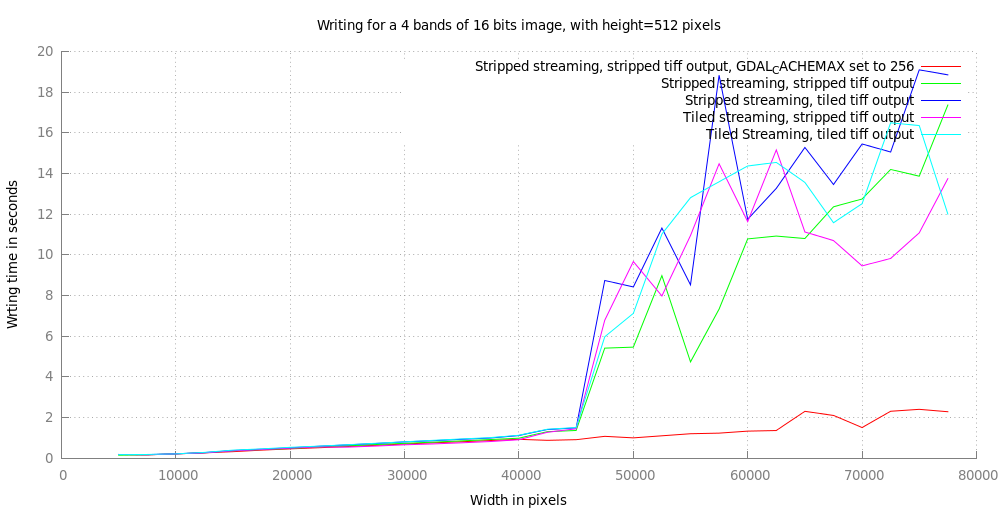
\includegraphics[width=\textwidth]{images/Writing.png}\\
\tiny{Effect of image encoding on image processing}
\end{center}
\end{frame}

\begin{frame}
\frametitle{Support/Help/Contribute}
\vspace{-0.2cm}
\begin{block}{General resources}
\vspace{-0.2cm}
\begin{description}
\item[Site web] \href{http://www.orfeo-toolbox.org}{orfeo-toolbox.org}
\item[Wiki] \href{http://wiki.orfeo-toolbox.org}{wiki.orfeo-toolbox.org}
\item[Blog] \href{http://blog.orfeo-toolbox.org}{blog.orfeo-toolbox.org}
\end{description}
\end{block}
\vspace{-0.2cm}
\begin{block}{Documentation and help}
\vspace{-0.2cm}
\begin{description}
\item[Guides] Software Guide and CookBook (remote sensing recipes)
\item[Doxygen] \href{http://www.orfeo-toolbox.org/doxygen}{doxygen}
\item[Users mailing list] otb-users@googlegroups.com
\item[Developers mailing list] otb-developers@googlegroups.com
\end{description}
\end{block}
\vspace{-0.2cm}
\begin{block}{Follow-up}
\vspace{-0.2cm}
\begin{description}
\item[Look at the code?] \href{http://git.orfeo-toolbox.org}{git.orfeo-toolbox.org}
\item[Find a bug?] \href{http://bugs.orfeo-toolbox.org}{bugs.orfeo-toolbox.org}
\item[Agile?] \href{http://scrum.orfeo-toolbox.org}{scrum.orfeo-toolbox.org}
\item[Weather?] \href{http://dash.orfeo-toolbox.org}{dash.orfeo-toolbox.org}
\end{description}
\end{block}
\end{frame}


\begin{frame}
\frametitle{Thank you! Any questions?}
\begin{minipage}[t][6cm][t]{\textwidth}
\begin{center}
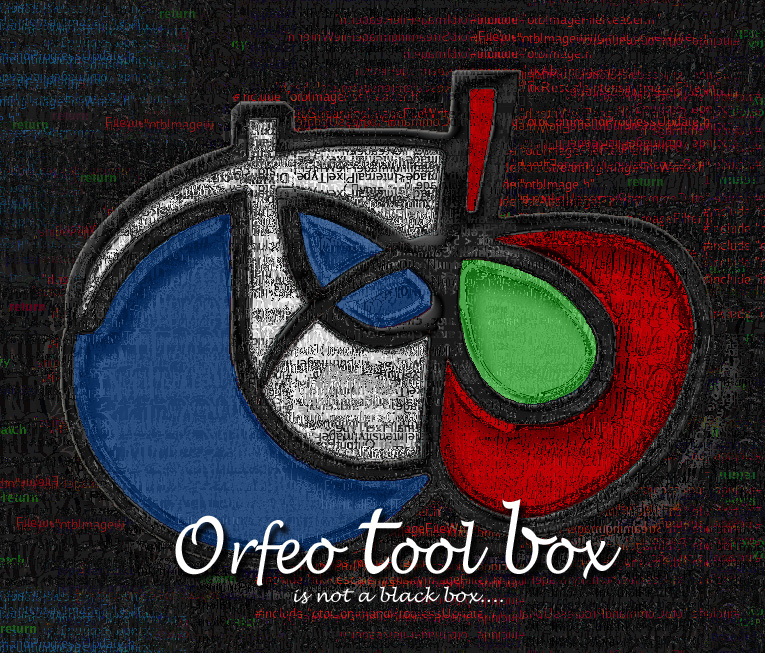
\includegraphics[width=0.65\textwidth]{images/LOGOTB_blackbox.png}
\end{center}
\end{minipage}
\end{frame}

\end{document}
